\section{Introduction}
% a contextual description of the goals of experiment

In 1921, Michelson and Peace developed the concept of {\it astronomy interferometry} \cite{michel}, measuring the {\it angular diameter} of one the brightness star in the sky, {\it Betelgeuse}, with an {\it optical telescope}. Nowadays,  Michelson and Peace techniques have broad applications in astronomy to measure stellar diameters \cite{sbu}.

{\it Optical} (wavelength ranges of 390 to 750 nanometers) or {\it Radio interference} (wavelength range of hundreds of meters to millimeters) \cite{wiki} can be achieved by superimposing signals from more than one telescope, yielding superior {\it resolutions} than that offered by the telescope alone \cite{brand}. This is due the fact that the orders of magnitude of the wavelengths in the radio electromagnetic spectra are scalables to the {\it baselines distances}. Interferometry is a powerful tool in radio astronomy. 

A {\it radio interferometer} measuring an extensive source such as the Sun will show a proportional relation of the dimensions of the experiment (\ie measurable baseline lengths), to the radio wavelength detected, and  to the {\it sizes of fringe}, in the resulting power spectra. In addition, precise values for the baseline lengths can be inferred by observing the power spectra of a point source (\eg an artificial geostationary satellite).

In our experiment, we make use of a two-mirrors  radio interferometer, assembled in the Stony Brook University\cite{sbu}, to measure the angular diameter of the Sun, $\Phi_{sun}$. We show that the Sun is roughly resolved when viewed in {\it single-dish mode}, but it is well resolved when {\it observed interferometrically}. 
\bigskip


\subsection{The Geometry of Radio Interferometry}

The principle of {\it superposition of waves}, figure \ref{int}, states that when two or more waves are incident on the same point, the {\it total displacement} at that point is equal to the {\it vector sum of the displacements of the individual waves}. If a crest of a wave meets a crest of another wave of the same frequency at the same point, the {\it magnitude of the displacement} is the {\it sum of the individual magnitudes}, yielding a {\it constructive interference}. If a crest of one wave meets a trough of another wave, the magnitude of the displacements equals the difference in the individual magnitudes, yielding a {\it  destructive interference} \cite{brand}.

\begin{figure}[htb]
\begin{center}
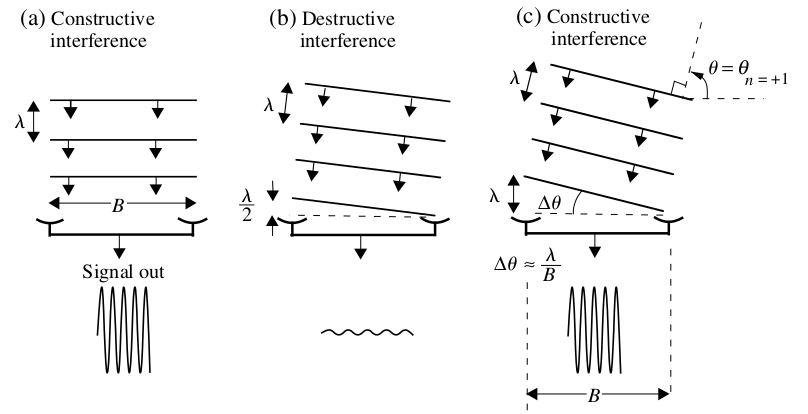
\includegraphics[scale=0.55]{figs/inter.png}
\caption{Interference between two plane wave from a distance source at different angles, from \cite{brand}. The signals are vectorially added, constructively (a), (c), and destructively  (b). }
 \end{center}
\label{int}
\end{figure}



An interferometer will detect and vectorially add signals from two different positions, figure \ref{fig:t}-a. The signal arrives on the two {\it mirrors}, being then mixed in the {\it antenna receiver}. The separation between the two positions (mirrors) is named {\it baseline length}, $B$.

\begin{figure}[htb]
\begin{center}

 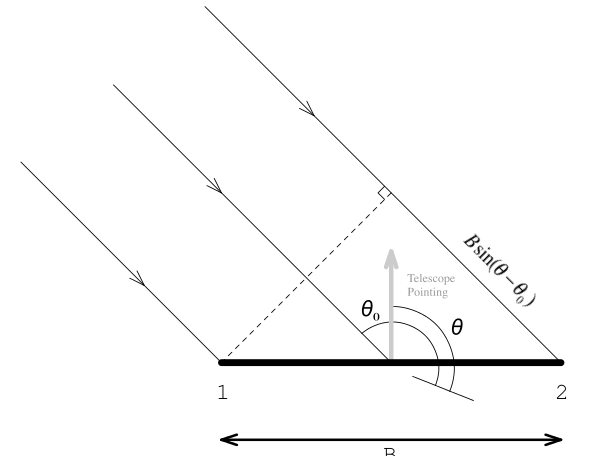
\includegraphics[scale=0.45]{figs/time.png}  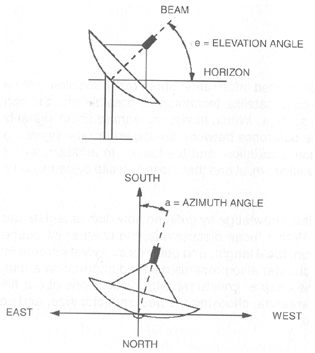
\includegraphics[scale=0.81]{figs/ele.jpg}
\caption{(left)  a -  Signal detection on two mirrors on a radio telescope separated by a baseline length $B$, from \cite{sbu}. (right) b - Elevation and azimuth angles in the dish.}
\label{fig:t}
 
\end{center}
\end{figure}


From an arbitrary origin, we define the horizontal variable angle of the telescope pointing, $\theta$, and the fixed horizontal angle coordinates of the object in the sky, $\theta_0$, as in figure \ref{fig:t}. The angle $\theta_0$ will be later related to the actual azimuth, $A$, of the object. It will be also useful to calculate the {\it declination}, $\delta$ of the object (equatorial coordinates), that can obtained from the {\it elevation}, $E$, the {\it azimuth}, and the geographical latitude $\phi$ (horizontal coordinates)\cite{wiki},
\begin{equation}
\sin \delta = \sin \phi \cdot \sin E + \cos \phi \cdot \cos E \cdot \cos A.
\label{dec}
\end{equation}



The signal wavefronts arrive at the telescope in phases because one of the sources is overhead. The {\it time delay}, $\tau$, of the signal at the position 2 (figure \ref{fig:t}-a), is related to difference between these two angles, the baseline length $B$, and the electromagnetic radiation speed, {\it c},
\begin{equation}
\tau = \frac{B \sin(\theta - \theta_0)}{c} \approx \frac{B(\theta - \theta_0)}{c},
\label{t}
\end{equation}
where we use the fact that $\theta-\theta_0\ll1$, such that the Taylor-expansion for small-angle approximation allows $    \sin \theta \approx \theta $.

\bigskip

\subsection{The Physics of Radio Interferometry}

Electromagnetic radiation can be written in terms of their perpendicular {\it electric fields, E}, and {\it magnetic fields, B}, where the last can be simply derived from the first with the {\it Maxwell Equations} \cite{jackson}.

The radio signal is electromagnetic radiation. At the frequency $\nu$, its time-sinusoidal amplitude arriving at position 1 (figure \ref{fig:t}-a) can be described as a plane wave with the  electric field  amplitude \cite{sbu},
$$\mathbf E_1(t) = \mathbf E(\theta_0)   \cos [2\pi \nu t] .$$

The signal arriving at position 2 at that same time has traveled $B \sin(\theta - \theta_0)$ more than $E_1(t)$, and its electric field amplitude  is
$$\mathbf E_2(t) =  \mathbf E(\theta_0)  \cos [2\pi \nu (t-\tau)] .$$



In the  interferometer receiver, the two signals are vectorially added,
$$
\mathbf E_{tot}(t) =  \mathbf   E_1(t) + \mathbf E_2(t),
$$
 and the receiver detects the {\it total power} of the signal, $P(t)$.  The radio frequency, $\nu$, is large compared to a data sampling rate of the receiver, and the total power detected  is {\it time averaged} (or integrated) \cite{sbu} \cite {brand} \cite{jackson},
\begin{eqnarray}
P(t) &=& \langle\mathbf E_{tot}(t)^2 \rangle, \nonumber \\
& =&   E^2(\theta_0) [1+ \cos (2\pi \nu \tau)],  \nonumber \\ 
P(\theta)&=& E^2(\theta_0) [1+ \cos (2\pi B_{\lambda} (\theta - \theta_0))],
\label{p}
\end{eqnarray}
where 
$B_{\lambda} \equiv B/\lambda,$ 
is the {\it normalized baseline length} to the wavelength $\lambda = c/\nu$ and we have applied the results from equation (\ref{t}).

Considering that the object has an extension in the sky,  we can rewrite equation (\ref{p}) as a continuum total power law,
\begin{eqnarray}
P(\theta) = \int \varepsilon (\theta_0) d\theta_0 \Bigg [1+ \cos \Big (2\pi B_{\lambda} (\theta - \theta_0)\Big)\Bigg ].
\label{p22}
\end{eqnarray}

An astronomical object can have any kind of structure, this will result on many kinds of the {\it energy density distribution},  $\varepsilon(\theta_0)$. The telescope interferometer receiver will measure the  sinusoidal power intensity response of the object given by equation (\ref{p22}), where $\theta$ are the fringes pattern due the interferometry. This quantity will be directly related to the {\it Fourier transformation} of the energy density distribution of the object.

\bigskip



\subsection{Obtaining the Baseline Lengths from a Point Source }



For a punctual source (artificial geostationary satellite), the energy density varying  on $\theta_0$ (as we sweep the telescope)  is a $\delta$-function at the position of the object:
\begin{eqnarray}
 \varepsilon_{sat} (\theta_0) = \varepsilon_0 \delta (\theta_0). 
\label{del}
\end{eqnarray}

An expect profile of the total power (amplitude squared) of a point source measured interferometrically can be seen in the figure \ref{bas}. The pattern of this figure can be thought as resolved  as a serie of point sources, slightly displaced, where the interference and the peaks and valleys shrink towards the central value of one. 


We insert equation (\ref{del}) into (\ref{p22}) and integrate. As we have mentioned in the beginning of this session,  measurements of a point source yields the accurate measurement of  baseline lengths. The total power is zero in the fringe's minimums (destructive interference, as shown in the figure \ref{int}), becomes
\begin{eqnarray}
P_{sat}(\theta) = \varepsilon_0  \Bigg [1+ \cos \Big (2\pi B_{\lambda} (\theta - \theta_0) \Big ) \Bigg] \equiv 0,
\label{p223}
\end{eqnarray}
meaning
\begin{eqnarray}
2\pi B_{\lambda} (\theta - \theta_0) & =& (2n+1) \pi  \nonumber \\
B_{\lambda} (\theta - \theta_0) & =& \frac{2n+1}{2}. \nonumber
\end{eqnarray}

Therefore, the separation between adjacent null positions (\ie the {\it angular size of the component} we are measuring) gives the value of the baseline lengths,
\begin{eqnarray}
B_{\lambda} \Delta \theta_{12} &=& \frac{2(n_1 - n_2)}{2},\nonumber \\
B^{\Delta \theta}_{\lambda} &\approx& \frac{1}{\Delta \theta}.
\end{eqnarray}
(as we can observe, again in the figure  \ref{bas}). We say it is an approximate value because the rotation of the earth plays a role here, it continuously reorients the telescope, causing the directions of the constructive/destructive interference to scan across the radio source. For instance, the earth rotates $0.5^o$ each every 2 minutes.  This oscillation/modulation should be at a much lower frequency than the radio frequency \cite{brand}.

\begin{figure}[htb]
\centering
 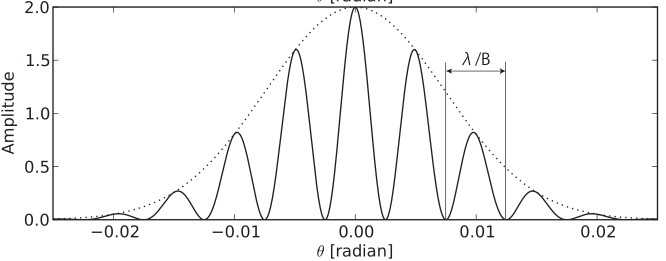
\includegraphics[scale=0.55]{figs/bas.png}
\caption{Example plot of total power as function of telescope pointing, $\theta$ for a point source such as the satellite, from \cite{sbu}. }
\label{bas}
\end{figure}


In addition, with the  actual  declination of the object, $\delta$, from equation (\ref{dec}), the fringe $\Delta \theta$ is the {\it Fourier transform} of the fringe period $\Delta t$.  Considering the angular frequency of earth rotation as $\omega = 15^o / h$, we can also obtain the baseline lengths writing 
\begin{equation}
  B^{\Delta t}_{\lambda} = \frac{1}{\cos(\delta) \sin(\omega \Delta t)}.
\label{BB}
\end{equation}

In the rest of this session, we shall write $B_{\lambda}$  for simplicity.




\bigskip

\subsection{Calculating the Angular Diameter of the Sun} \label{visb}


We can rewrite the total power given by equation (\ref{p22}),
$$ P_{sun}(\theta) = \int \varepsilon (\theta_0) d\theta_0 + \int \varepsilon (\theta_0) \cos (2\pi B_{\lambda} (\theta - \theta_0)) d\theta_0.$$

This is the the Fourier transformation of the object's energy density distribution and we can prove it rewriting the above equation in the same fashion as in \cite{sbu}:
$$P_{sun}(\theta) = S_{sun} [1+V(\theta,B_{\lambda})],$$
where
$$ S_{sun} = \int \varepsilon (\theta_0) d\theta_0,$$
is the full spectra of the Sun (obtained as a single dish rather than as interferometer), and
\begin{eqnarray}
V(\theta, B_{\lambda})&=& \frac{1}{S_{sun}} \int \varepsilon (\theta_0) \cos [2\pi B_{\lambda} (\theta-\theta_0)] d\theta_0 ,\nonumber \\
&=& V_{sun} (B_{\lambda}) \cos [2\pi B_{\lambda} \theta],
\end{eqnarray}
 where we gauge the {\it zero-phase position} of the coordinates to eliminate a phase. $V_{sun}$ is the visibility function of the Sun (an amplitude of the Fourier transform a baseline length $B_{\lambda}$),
\begin{equation}
V_{sun}(B_{\lambda}) = \frac{1}{S_{sun}} \int \varepsilon (\theta_0) e^{-i2\pi B_{\lambda} \theta_0}d\theta_0.
\end{equation}

We can compare this to the observed total power law,
$$P_{sun}(\theta) = S_{sun} \Big [1 + V_0(B_{\lambda}) \cos [2\pi B_{\lambda} (\theta - \Delta \theta)]\Big].$$

\bigskip

To extract the power function from an astronomical source, $P_{sun}(\theta)$, we sweep the object by changing the direction of the telescope pointing, $\theta$. We see a  sinusoidal curve plus an {\it offset} proportional to  $\theta$, as shown in the figure \ref{psun}, together with maximum and minimum values for the total power function.



\begin{figure}[htb]
\centering
 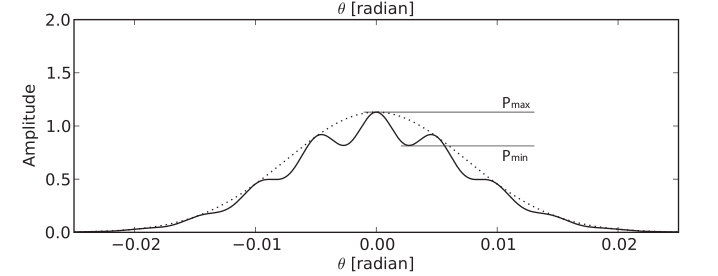
\includegraphics[scale=0.55]{figs/psun.png}
\caption{Example plot of total power as function of telescope pointing, $\theta$ for a extended source, such as the Sun, from \cite{sbu}. }
\label{psun}
\end{figure}

It is straightforward to rewrite out results in terms of $P_{max}$ and $P_{min}$,
\begin{equation}
P_{max} = S_{sun} [1 + V_{sun}(B_{\lambda})], 
\end{equation}
\begin{equation}
 P_{min} = S_{sun }[1-V_{sun}(B_{\lambda})].
\end{equation}

The {\it visibility function}  is then
\begin{eqnarray}
V_{sun}(B_{\lambda}) &=& \frac{P_{max} - P_{min}}{P_{max} + P_{min}}.
\label{vis}
\end{eqnarray}
which is a {\it sinc} function in term of  the baseline lengths,
\begin{eqnarray}
V_{sun}(B_{\lambda}) &=& \frac{\sin  ( \pi   B_{\lambda} \Phi_{sun}  )}{ \pi B_{\lambda} {\Phi_{sun}}}, \nonumber \\
&\equiv& \mbox{ sinc } (B_{\lambda} {\Phi_{sun}}).
\label{vissinc}
\end{eqnarray}


In this experiment we apply  these properties of the visibility function as a Fourier component of our measurement to obtain the final values of the angular diameter of the sun.


